\documentclass[twocolumn,a4paper,10pt]{article}
\usepackage{graphicx}
\author{DongWei Zhou}
\title{GPSA:A Graph Processing System with Actors}
\begin{document}
\maketitle
\section{Abstract}
Graph-based applications become hotter and hotter due to the rising of the social-networks and other problems come up such as paths of disease outbreaks, or chemical compounds, or biological structures. A strong desire to process large graph motivates researchers to study on distribute memory machines. Unfortunately, developing distributed graph algorithm still requires some cost, especially to non-expert. While manufacturing technology improves, physical limits of semiconductor-based microelectronics have become a major design concern. A combination of increased available space and the demand for increased thread level parallelism led to the development of multi-core CPUs. Today, a single multi-core server already has a very powerful computing capabilities, which means we can exploit its capabilities to do more job.
In this paper, we present GPSA, a graph processing system with actors on a single machine. We worked on the computation model of graph processing with actors, which could process the message in a more natural method. And also we avoid the consumption caused by the frequent switching among threads. And last, in order to reduce the influence may caused by I/O, we utilize the memory mapping for better performance. We show, through experiments and theoretical analysis, that processing large-scale graph on a modern PC with actors performs well.

\section{Introduction}
Graph algorithms are becoming increasingly important for solving many problems in scientific computing, data mining and other domains such as social networks, web graphs, chemical compounds, and biological structures. The scale of real graphs is so large that may consist of billions of vertices, trillions of edges. For Example, the Yahoo Web graph have 1.4 billion vertices and 6.6 billion edges. However, Graph processing is difficult because of the inherent complicated data structure of the graph and the extremely large size of the graph. Therefore, designing a scalable, fault-tolerant, robust system for processing the large-scale graphs is one of the most urgent problems facing systems researchers.
\newline
Motivated by the demands, there are already some solutions, which are able to process large scale graphs with distributed system such as Pregle, PowerGraph and GPS, proposed by other researchers. Nowadays,though distributed computional resources are more accessible than ever before, processing these graphs still remains many challenges. In distributed system, the first main problem is workload balancing which caused by partitioning the large scale graph into small partition to fit the cluster nodes. The second main issue is message passing. Messages exit among the different computional nodes or inside of the cluster node, the cluster nodes take cost to communicate with each other and the communication between nodes causes latency which matters in a BSP based graph processing system.Therefore, many researchers spend a lot of energy to study the distributed system based on Pregel to solve the problems mentioned above and some gain reasonable performance, such as Mizan which aims to the workload balancing, GPS focus on the messaging latency. But from a developer’s perspective, developing, debugging and optimizing distributed algorithm on distributed system is quite difficult because the user needs to be skilled at managing and tuning a distributed system in a cluster, which is a nontrivial job for the ordinary user. Besides, these distributed systems need many machines in a cluster which brings both money and energy cost.
\newline
Recently, some graph processing engines on single PC have been proposed to address the problems of the distributed graph systems. For example, Ligra is a lightweight graph processing framework this is specific for shared-memory multi-core machine. Specially, Graphchi, a disk-based graph processing engine on a single modern PC, significantly outperforms all representative distributed graph engines. TurboGraph inspired by Graphchi focuses on parallelism and overlapping of CPU processing and I/O processing with a novel concept pin-and-slide.
\newline
However, we observe that none of the existed single PC engine underultilize the resource of the multi-core machine or the operating system. Parallelism could improve the computing efficiency. Given the success of parallel computing in scientific computing, data analysis and other areas, parallel processing appears to be necessary to overcome the resource limitations of single processors in graph computations. While the inherent complicated characteristics of the graphs make them hard to match the current parallelism computational problem-solving approaches. Vertex-centric is a very brilliant idea for graph processing. In the mode, every single vertex is a little compute unit, which simplifies the process, and every vertex communicate with each other by message. Unfortunately, a modern PC could not support a large number of concurrent, because the concurrent implemented by thread has its limitation. Motivated by this issue, we present a totally different graph processing engine on a single modern PC. We implements the engine with actor/coroutine, actor/coroutine is anultra-lightweight thread thatcould greatly improve concurrency. The higher the concurrency, the more suitable the vertex-centric is. We are bold attempt to map a vertex to an ultra-lightweight thread and transfer the communication between vertices into the communication of ultra-lightweight thread. Besides, we notice that the IO processing is the main efficiency killer, we exploit the ability of memory mapping provided by the operating system.
\newline
The rest of the paper is as follows. Section 2 reviews related work. In next section, we adopt the vertex-centric model to fit the ultra-lightweight thread and show the difference. Section 4 presents the detailed implementation of the engine. Section 5 describes the experiments results. And in section 5, and section 6 summarizes and concludes the paper.

\section{Related Work}
Many scalable graph systems have recently been proposed. We survey some of the most relevant works, which may be broadly classified into single-machine approaches and distributed approaches depending on the size of the system.
\newline
	Distributed Systems: Pregel is a synchronous vertex-centric programming model proposed by Google for graph system. In Pregel, each vertex is executed in parallel and the user rewrite the compute function invoked by the vertex. Pregel introduced the first bulk synchronous parallel (BSP) distributed message-passing system. In BSP model, all vertex kernels run simultaneously in a sequence of super-steps. Within a super-step, each vertex receives messages from in-neighbor of the last super-step and sends messages to out-neighbor of the next super-step. And a barrier is imposed between two super-steps to guarantee that all vertices finish processing messages.However, Pregel is not open-source and many other systems drown from Pregel such as GPS, PowerGraph, GraphLab, Mizan etc. Other systems Pegasus and gbase are based on MapReduce and support matrix-vector multiplication using compressed matrices.
\newline
Single-machine Systems:X-Stream is a system for processing both in-memory and out-of-core graphs on a single shared-memory machine. X-Stream take advantage of using an edge-centric model and streaming completely unordered edge lists rather than performing random access. Ligra is a lightweight graph processing framework this is specific for shared-memory multi-core machine. Graphchi is a disk-based single-machine system following the asynchronous vertex-centric programming model. Graphchi proposed parallel sliding windows (PSW) to handling disk-based large-scale graphs and it updates values to the edges in Graphchi. PSW partitions the vertices into P execution intervals, and each execution interval contains a shard file that stores all in-edges sorted by their source vertices. PSW processes one shard at a time. During the processing, first of all, loading an execution interval into memory from the disk, then update the vertices and edges. At last, writing the updated content to disk.

\section{Overview}
While manufacturing technology improves, reducing the size of individual gates, physical limits of semiconductor-based microelectronics have become a major design concern.A combination of increased available space (due to refined manufacturing processes) and the demand for increased thread level parallelism (TLP) led to the development of multi-core CPUs. Since the multi-core has already become the main architecture of the modern PC, in theory, the modern PC should have a powerful computional ability. However, the concurrent computing is still not mature which causes underutilization of the multi-core machines. There are main two ways to implement concurrent computing, multi-process and multi-thread. However, in a single machine, the number of process or thread has its limitation which means poor concurrency and concurrent with thread invoke locks and synchronous. In fact, there is another concept called actor.
\newline
The actor model is a different way of modeling concurrent processes. Rather than threads interacting via shared memory with locks, the actor model leverages "actors" that pass asynchronous messages using mailboxes. A mailbox, in this case, is just like one in real life — messages can be stored and retrieved for processing by other actors. Rather than sharing variables in memory, the mailbox effectively separates distinct processes from each other. Actors act as separate and distinct entities that don't share memory for communication. In fact, actors can only communicate via mailboxes. There are no locks and synchronized blocks in the actor model, so the issues that arise from them — like deadlocks and the nefarious lost-update problem — aren't a problem. What's more, actors are intended to work concurrently and not in some sequenced manner. As such, actors are much safer (locks and synchronization aren't necessary) and the actor model itself handles coordination issues. In essence, the actor model makes concurrent programming easier. The actor model facilitates concurrent programming by allowing a safer mechanism for message-passing. Implementations of this model vary between languages and frameworks. Luckily, there are a number of choices for leveraging this model on the Java platform.

\subsection{Actor of Kilim}
Kilim is a library written in Java that embodies the actor model. In Kilim, "actors" are represented by Kilim's Task type. Tasks are lightweight threads and they communicate with other Tasks via Kilim's Mailbox type. Mailboxes can accept "messages" of any type. Tasks can send String messages or even custom message types — it's entirely up to you. Everything is tied together in Kilim via method signatures; if you need to do something concurrently, you specify the behavior in a method by augmenting its signature to throw Pausable. Thus, creating concurrent classes in Kilim is as easy as implementing Runnable or extending Thread in Java. At last, Kilim's magic is enabled by a post process, called a weaver, which alters the byte code of classes. Methods containing the Pausable throws clause are processed at runtime by a scheduler, which is part of the Kilim library. The scheduler manipulates a limited number of Kernel threads. It is able to leverage this pool for a higher number of lightweight threads, which can context-switch and start up quite fast. Each thread's stack is automatically managed. The actor model makes it easier and safer to write asynchronous-acting objects that depend on similar objects.

\subsection{Model of Computation with Kilim}
The vertex-centric programming model introduced by Pregel is based on the Bulk Synchronous Parallel (BSP) computation model. As mentioned above, BSP consists of a sequence of super-steps and a barrier is imposed between two super-steps. Within super-step, all vertices kernels run simultaneously. Receiving messages from the last super-step, invoking the user defined computing method, updating the value of the vertices and sending messages to the next super-step. While in a actor, there are no super-steps in conceptually, there is a biggest common thing that both of them involved: message passing.
\newline
To implement a BSP model with actor is quite smoothly, because the similarity of vertex-centric programming model and actors. Image that each vertex is an actor and the communication among vertices,in fact, transferring into the communication among actors, which is a very nature thing. However, BSP seems to be more suitable for distributed system because it is simple to implement and allows maximum level of parallelism without the concern of shortage of memory resource during the computation. Besides, every vertex kernel cannot execute simultaneously because of the size of memory and the number of cores of the CPU on a single PC. So does the actors. So even it is the most nature way to implements a BSP model, however, on a single PC is still a challenge.
\newline
Here is our BSP computation model with actors that drawn from Vertex-centric and BSP model: we assume that vertices are the data carriers and the actors are the basic computational unit and all the message passing among vertices via actors. Instead of storing the messages or combining messages for the next superstep, the worker actors consume the messages immediately once the actors receive the messages. By that way, there is a little different from the traditional BSP model. When an actor need to send a message, it does not have to wait for the computation of the current iteration to finish and send the messages directly because the computation for the current iteration has already been finished in the last iteration.
In our model, we arrange our actors in hierarchy. At the bottom is the worker actors and its child actors which is the main computational unit. While upon the worker actors is the manager actors who is responsible for loading data from the disk, distributing task and synchronizing between super-steps.
\newline
We choose the actor model for the graph computation purpose for two reasons. First, the very common nature between vertices and actor which means we can simulate the graph computation in a more specific way . Second, context switch among actors is more light than that among threads. Third, we thought that there is also a potential asynchronous model with actor exists.

\begin{figure}[htbp]
\centering
 \begin{minipage}[]{1.4\textwidth}
     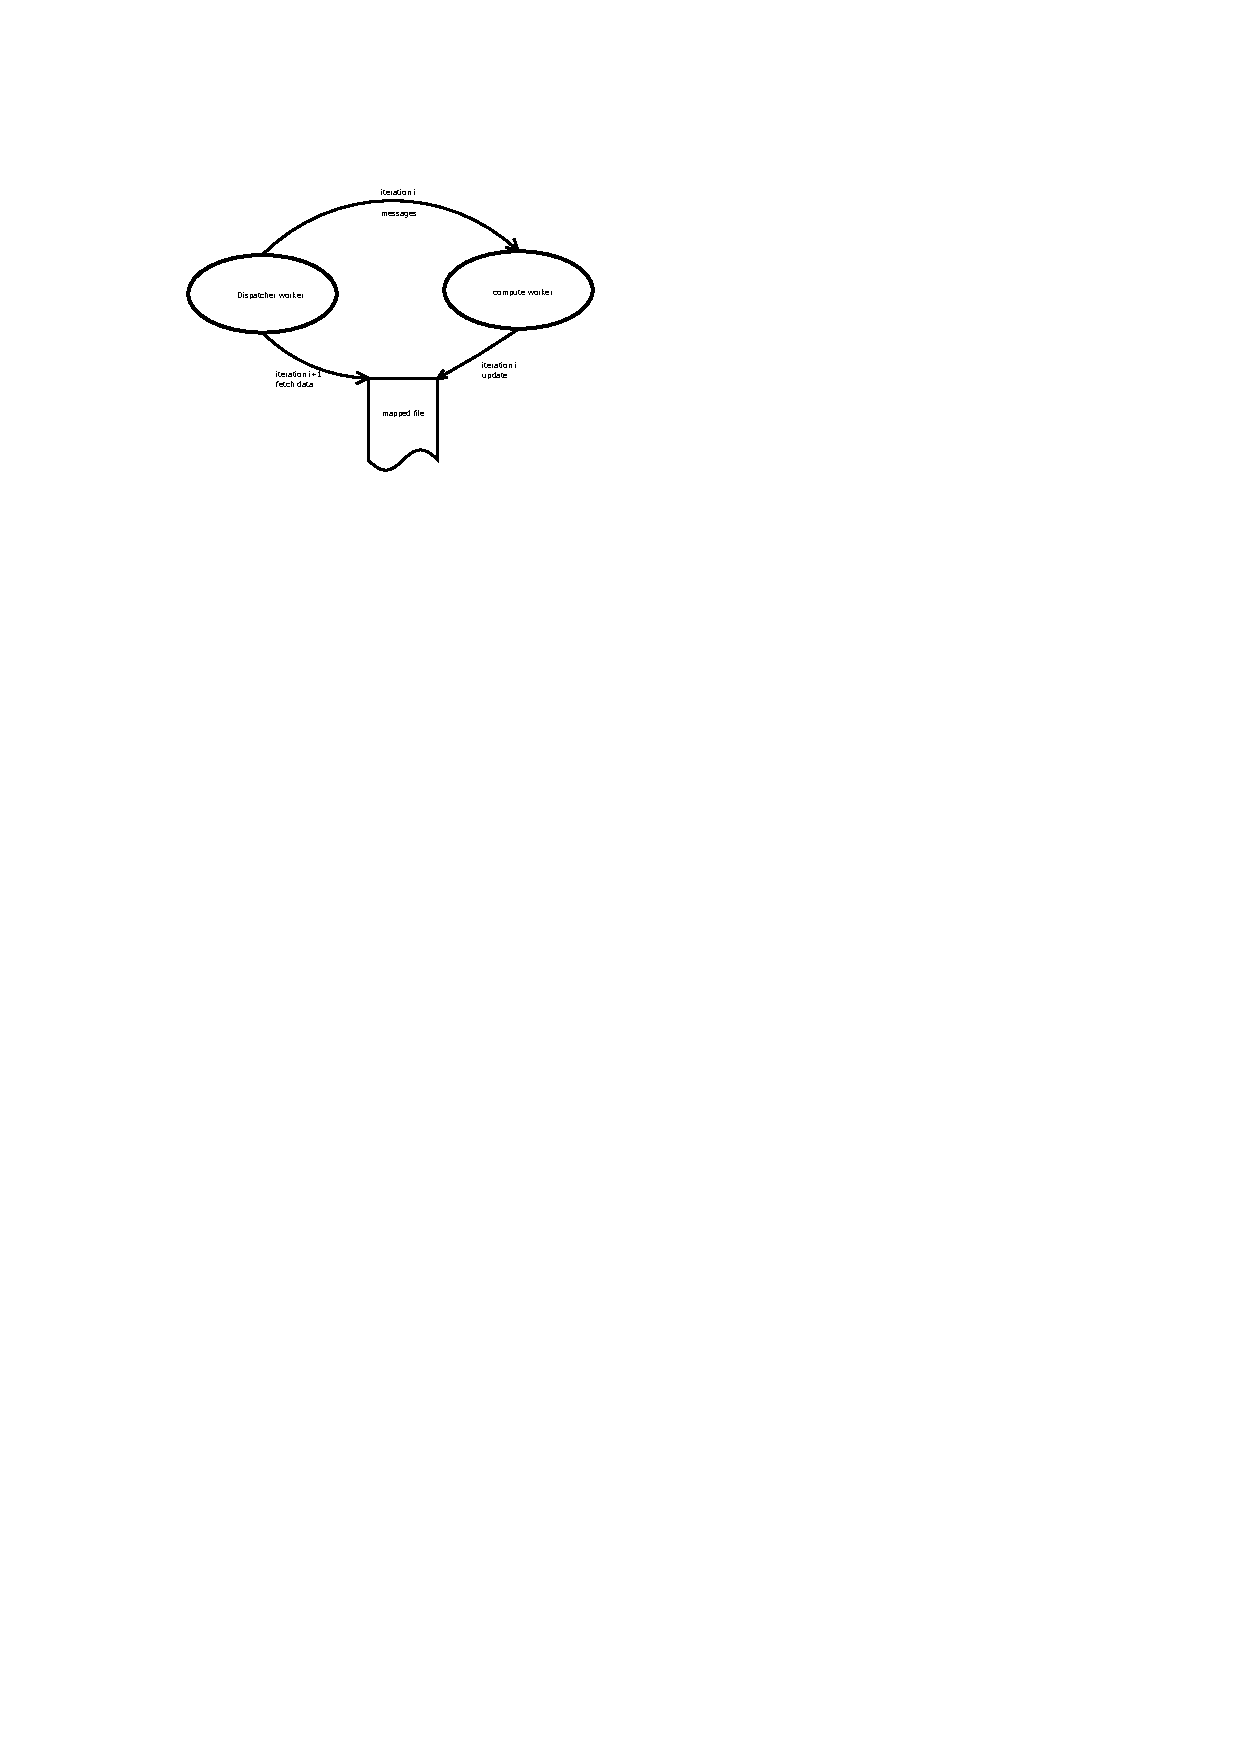
\includegraphics[width=0.4\textwidth,angle=0]{figure/computemodel.pdf}
\end{minipage}
    \caption{compute model with actors}
\end{figure}

\subsection{Asynchronous Model with actor}
Asynchronous computation model has been studied by many researchers. Asynchronous computation model means that all the vertices subsequently participate in the computation could be able to use the most recently values. So for two vertices, for example, Vj and Vk, if Vj processed before Vk , then the update of Vj should be visible by Vk , which means that the messages send from Vj to Vk will be replaced by the most recently messages. While for these two vertices, if they are processed by the same actor, then the sequence of the computation is certain, while if they are not, that will be unpredictable. And because of this indeterminacy, there is a chance for a actor to compute a message from the same sender twice in one iteration. So if the compute procedure is reversible, then we can recover the value from its last computation after the newer messages coming.

\section{Implementation}

\subsection{Memory Mapping}
The primary benefit of memory mapping a file is increasing I/O performance, especially when used on large files.Memory-mapping is a mechanism that maps a portion of a file, or an entire file, on disk to a range of addresses within an application's address space. The application can then access files on disk in the same way it accesses dynamic memory. Accessing memory mapped files is faster than using direct read and write operations for two reasons. Firstly, a system call is orders of magnitude slower than a simple change to a program's local memory. Secondly, in most operating systems the memory region mapped actually is the kernel's page cache (file cache), meaning that no copies need to be created in user space.\newline
The principal benefits of memory mapping are efficiency, faster file access, the ability to share memory between applications, and more efficient coding. Another benefits of memory mapping is we can access the data like an array. Mapping a file into memory allows access to data in the file as if that data had been read into an array in the application's address space.	\newline
In the 32-bit operating systems, memory-mapped files is usually used for high speed disk access. However, due to the limited address space of the 32-bit operating system, memory-mapped file is less likely used for massive virtual memory or for large files. While in a 64-bit operating system, memory-mapped files can map TB or even PB of memory into a process’s address space.  Fortunately, now that the JVM is 64-bit and could runs on 64-bit operation system, the JAVA developer doesn’t need to consider the disk and the memory as being separate things and could combine them with memory-mapped files via the MappedByteBuffer class. With memory-mapping, the process does not need to bother itself about whether the memory is in RAM or on the disk. The operating system takes care of that which is very fast. In order to utilize this feature of the
\subsection{Fault tolerance}
Fault tolerant is very important to guarantee the reliability of the system, especially for the high-performance demands. For a graph processing system, a fault-tolerant system must keep track of the whole state of the graph. However, keep so much information on a single commodity PC could be a burdensome of the system. So we take a compromise way, we separate the frequency changed data from the less frequency changed data and keep a backup of the most frequency changed data. For example, in a PageRank application, vertex value is more likely to updated frequently while the edge value seems to be useless. So we can separate the vertex value from the edge value.\newline
As mentioned above, we take the vertex as the data carrier and the actor as the compute unit. Instead of keeping track of the actors, we only need to record which messages the actor is to process. In our framework, we take advantage of the off-heap storage technology to avoid the frequency GC problems. In off-heap space, mapped byte buffer created by the memory mapping is a intuition choice. With the memory mapped file, we put and read the data in a sequential way. In a superstep, an actor has two kinds of total different role. One role is producer which happens when the actor needs to send messages. Another role is consumer when the actor need to get messages. In the off-heap space, actor write the message into the byte buffer, this byte buffer stores all the messages. So the mapped file will slowly grow in size as more data is written into the buffer. Even though the size of the buffer may be exceed the available memory, the only constraint is the disk space. When the system crashed someway, the system check the backup data on the disk and find out the most recent available message data, vertex value data and the graph adjacency list data, resign the data to the actor and continue the computation.\newline
Actors are the computational units in their purest form. The main purpose of the actor model is to break down the large task into small tasks. During the processing, if an actor throws an exception, for the performance reason, the manager actor will handle the exception. If the manager actor also have no idea what to do with the exception, then this exception will report to the supervisor manager actor.

\subsection{Data Arrangement and memory mapping}

Similar to the GraphChi, we also assume that the vertices are labeled from 1 to |V|. For convenience, the vertices are assigned to the computation actors by mod. Though the number of actors is depends on your hardware, we suggest that the number of actors better be the power of 2. So we can quickly  figure out a vertex by which actor be processed. And each value of the vertex are stored in a memory mapped file in ascending order by its label. In this way, we can access the data in a sequential way like a normal array. \newline
Before the computing, there is a pre-process. During the procedure, the graph are separated into different parts according the inherent attribute of the data. For example, separating the most likely changed data from the least. And store these information in different file on the disk. In fact, in graph everything could be modified, updating a vertex value, removing or adding a edge, deleting a vertex from the graph. However, for particular application, there is a relative relationship, such as in a PageRank algorithm vertex value is more fugitive than its edge value.  For a graph, the vertex value is maybe the most unstable because of the frequency update. So as mentioned above, we store the vertex value in a memory mapped file. Given a vertex, whose id is k, its value is stored in the k*value.szie(). Instead of partitioning the graph into some intervals to fit the memory, we arrange the graph in a adj-format file stored on the disk. And map portion of the file into memory once a time. \newline
\subsection{System Core}
 When the data has already been mapped into memory, manager tells its workers that data is ready. And the workers will start fetching their data from the file at the certain position, which means they can read data full parallel. Unlike the traditional BSP model, we decouple the compute and the send method. At first, we keep two copies of the initialized values. In an iteration, the worker do mainly two things: dispatching messages and computing messages. Once get the data, the worker start its execution loop. During the loop, worker will dispatch the messages to the destination worker according to the out edges of the fetched data. Once another worker actor receive the message, it will directly compute the message with certain value and put the updated value into memory mapped file. In this way, the update function and send function has no relationship with each other in the current iteration. If the user don’t want to compute the message with value directly, we also provided a Hook method combine, which combine the messages, like Pregel did.

\subsection{Worker Actor}
Worker actor is the most important role of the system. They are the basic execution units. Inside a worker actor, there is another kind of actor which listening to the message receiving event. This actor is created by the worker actor , thus is the child actor. After the worker actor get its data to be process, the worker actor dispatches messages to other worker actors. And the child actor will finish the compute task for the next iteration asynchronously. Therefore, the worker actor actually do the message dispatching stuff while leaving its compute burden to its child actor. In this way, we can update the graph fully parallelly.\newline
A worker actor maintains a sequence of the vertex ID. According to the sequence, the worker actor will clearly know where and how to get next data entry. And at the start of a new iteration, the sequence will be reset to start over again. There are two different mailbox in each worker actor. One for the messages between worker actors, which is used for computing or dispatching purpose. The another one is used for the communication with the manager. The child actor can only access the mailbox for compute purpose. When other worker actors put messages in the mailbox, the child actor will process the message one by one until the manager intervene in. If there is no messages, the child actor will keep waiting until the end .
\subsection{Manager Actor}
The main responsibility of the manager actor is coordinating the computation, exception handling, worker monitoring. Each manager will keep track of the states of its own workers. When the computation start, the manager will send workers an ITERATION\_START signal and the worker who receive this command will start execution immediately. When a worker finish all its work in current iteration, it will inform the manager with a DISPATCH\_OVER signal. Once all the works send DISPATCH\_OVER signal to its manager, the manager knows time to get into next iteration and send ITERATION\_OVER signal to its workers. After the worker receiving this, the worker will know this is the last message of the current iteration. Then the worker will reply with a COMPUTE\_OVER signal. At the end, an OVER signal will kill all the worker actors and finish the job.


\end{document}
